

\section{Transaction Lifecycle and Data Flow}
\label{sec:transaction_lifecycle}

The transaction lifecycle defines how a synthetic user transaction moves through the proposed ZK-rollup benchmarking framework, from workload generation to Layer-1 settlement. This lifecycle is important because it identifies the points at which throughput, latency, proving overhead, data availability footprint, and finalization time are measured. The lifecycle spans both the data plane and the control plane of the prototype. The data plane is responsible for transaction processing, batching, execution, proving, and submission, while the control plane supports orchestration, configuration management, retry handling, contract-state control, and telemetry collection.

\begin{figure}[!htbp]
    \centering
    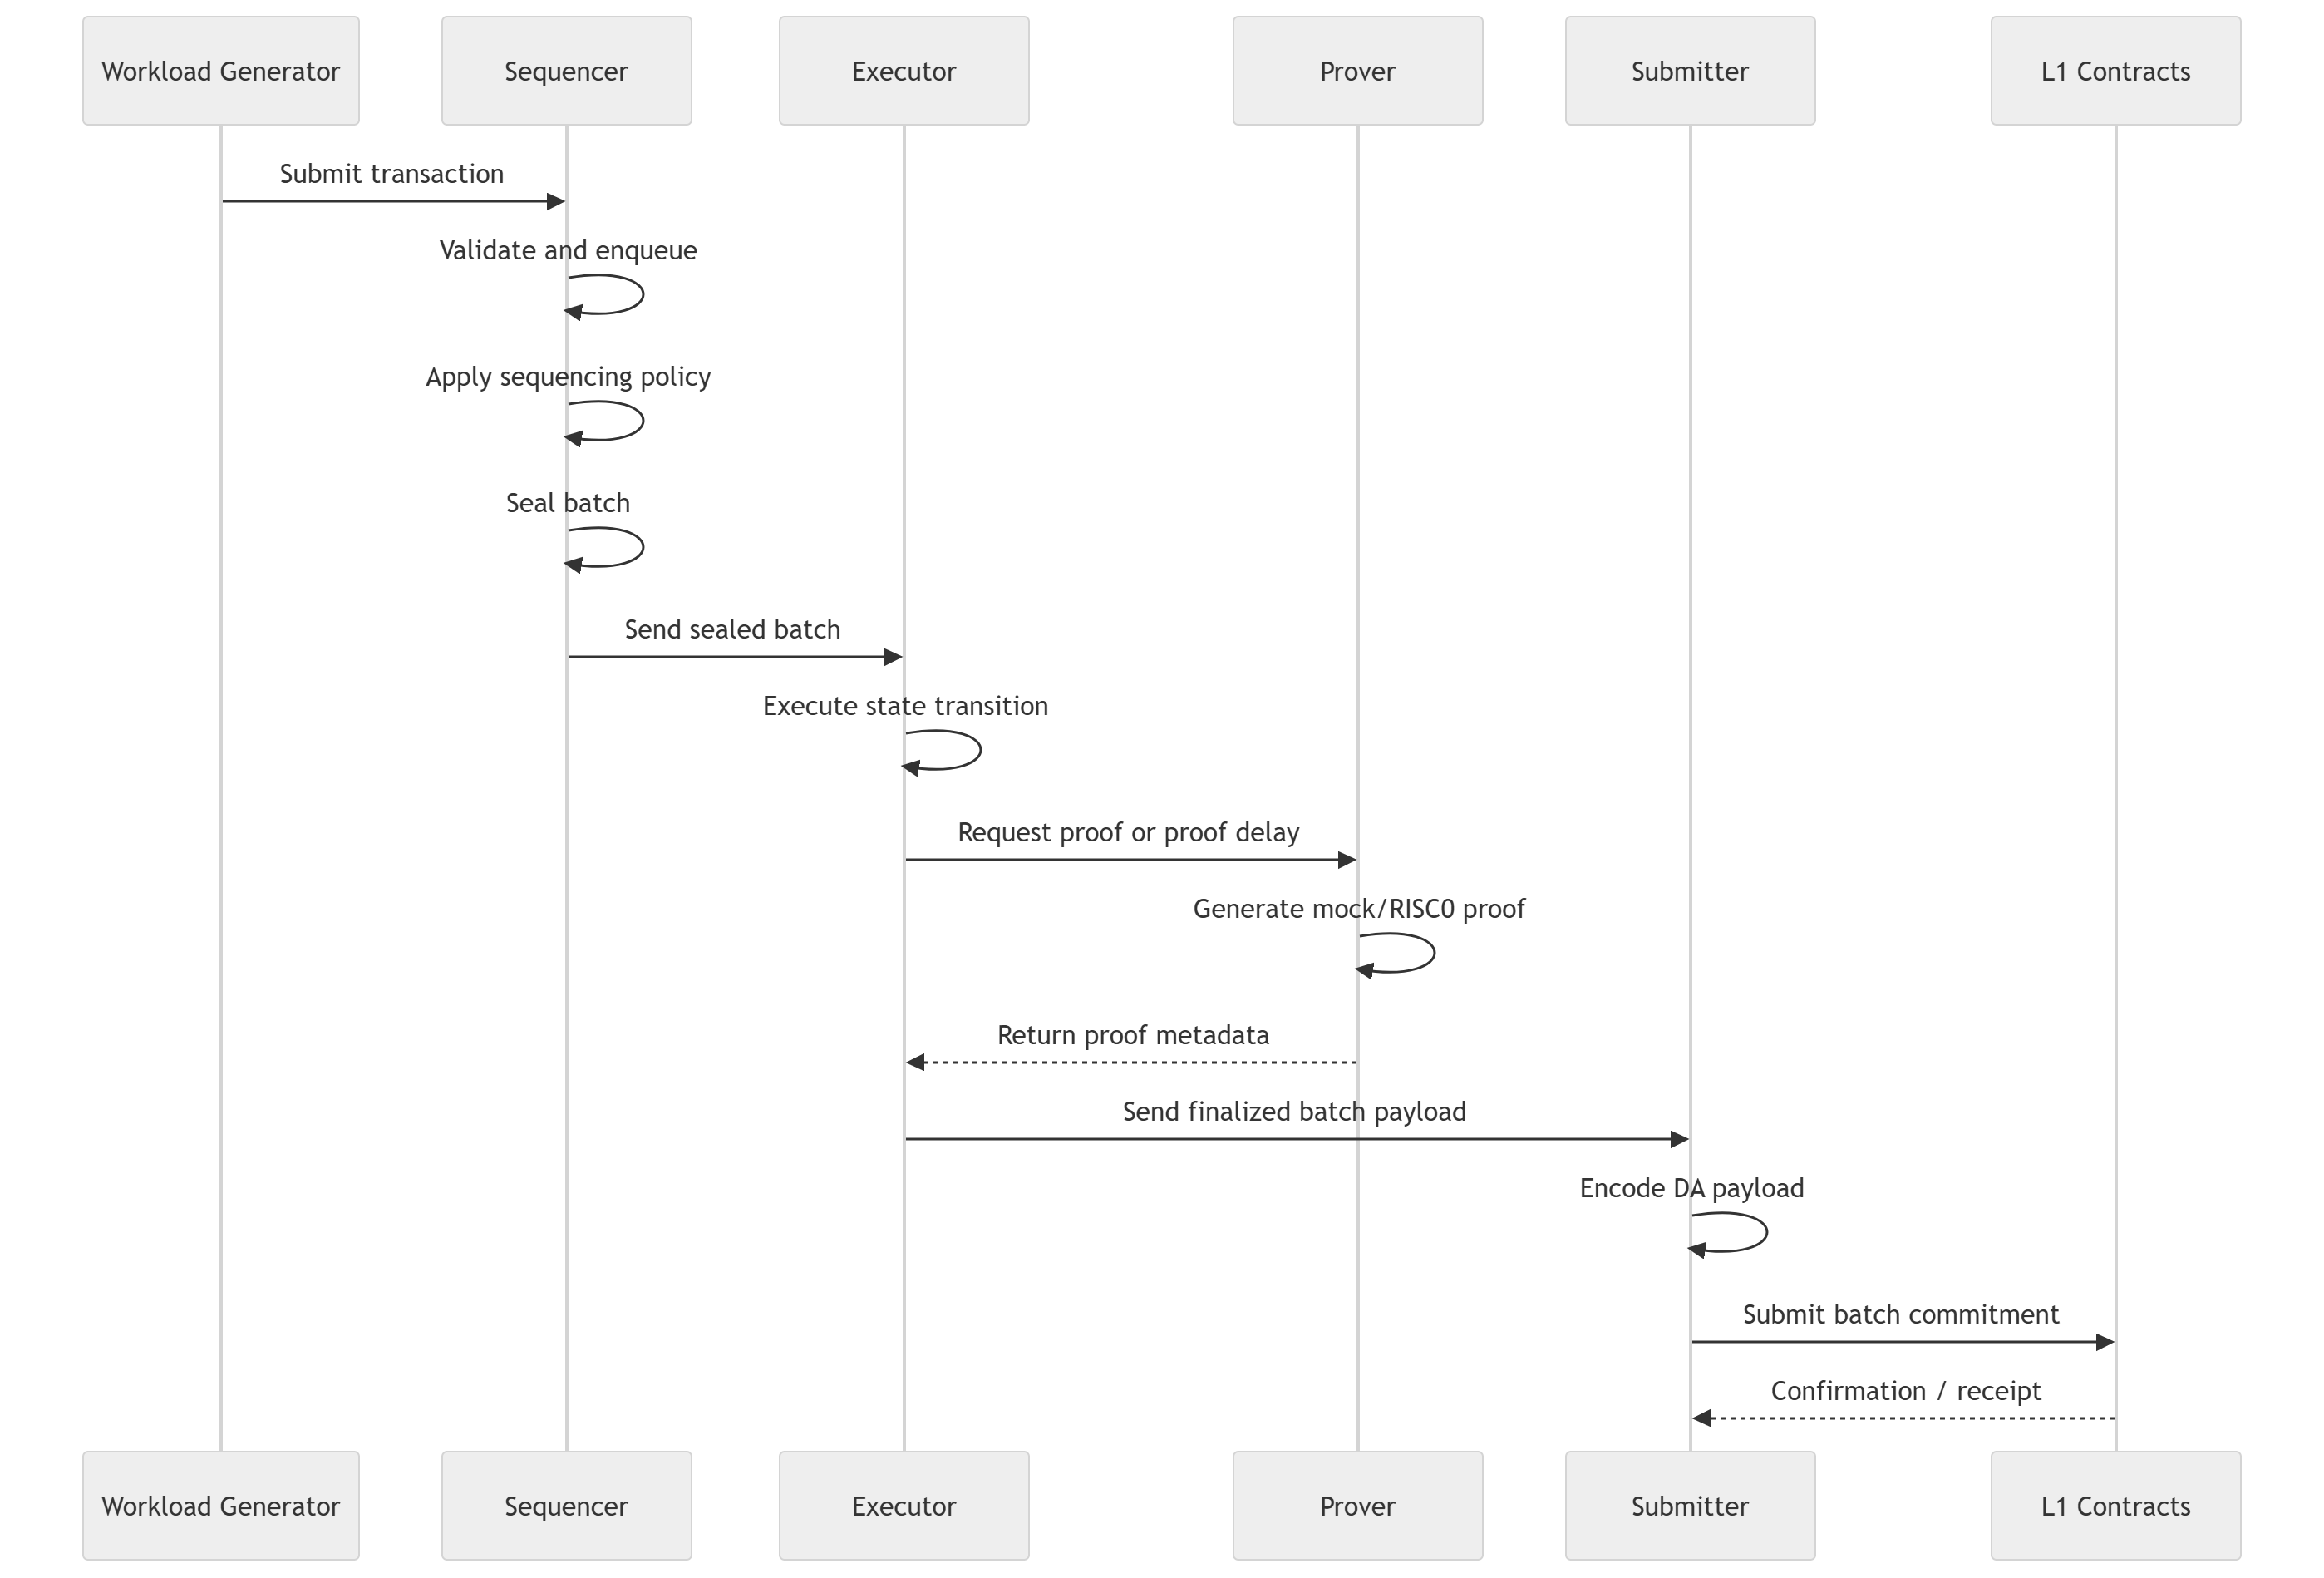
\includegraphics[
        width=0.98\textwidth,
        height=0.46\textheight,
        keepaspectratio
    ]{figures/chapter3/tx_flow.png}
    \caption{End-to-end transaction lifecycle through the RollupX framework.}
    \label{fig:transaction_lifecycle}
\end{figure}

Figure~\ref{fig:transaction_lifecycle} shows the main data flow across the RollupX pipeline. A synthetic transaction is generated by the Workload Generator and submitted to the Sequencer. The Sequencer validates and enqueues the transaction, applies the selected sequencing policy, and seals a batch once the configured batch-size or timeout condition is satisfied. The sealed batch is then forwarded to the Executor, which applies the state transition and requests proof generation from the Prover. After proof metadata is returned, the finalized batch payload is sent to the Submitter. The Submitter encodes the selected data availability payload and submits the batch commitment to the Layer-1 contracts. A confirmation receipt from Layer 1 marks the settlement point of the batch.

In addition to the transaction data flow, the Layer-1 contract layer includes a small control-state model that determines whether normal submission and forced-transaction handling are allowed.

\begin{figure}[!htbp]
    \centering
    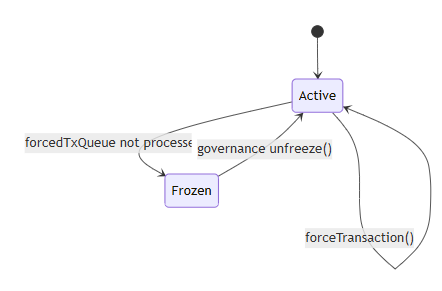
\includegraphics[
        width=0.48\textwidth,
        keepaspectratio
    ]{figures/chapter3/tx_lifecycle.png}
    \caption{Layer-1 contract state model for active and frozen execution modes.}
    \label{fig:l1_contract_state_machine}
\end{figure}

Figure~\ref{fig:l1_contract_state_machine} illustrates the simplified control-state behaviour of the Layer-1 contract. Under normal operation, the contract remains in the \textit{Active} state, where batch submission and transaction-forcing logic can proceed. If forced transactions remain unprocessed or the system enters an unsafe condition, the contract can transition into the \textit{Frozen} state. Governance-controlled recovery can then move the contract back to the \textit{Active} state. This model separates normal settlement behaviour from exceptional recovery behaviour.

The end-to-end transaction flow is described below.

\begin{enumerate}
    \item \textbf{Ingestion through the Workload Generator:}
    The Python-based Workload Generator creates controlled synthetic transaction traffic using a seeded Poisson arrival model. These transactions primarily represent transfer-style workloads and are submitted to the Sequencer through the configured API interface. This stage allows the same workload pattern to be reused across multiple benchmark configurations.

    \item \textbf{Sequencing and batching:}
    The Sequencer receives incoming transactions, performs validation, and stores valid transactions in a local transaction pool. It then orders transactions according to the selected scheduling policy, such as FCFS, FeePriority, or TimeBoost. A background batching engine continuously evaluates sealing conditions, including maximum batch size and timeout interval. Once a configured trigger is satisfied, the batch is sealed and forwarded to the execution stage. This point represents soft finality, where the transaction has been accepted into a rollup batch but has not yet been finalized on Layer 1.

    \item \textbf{Execution and state transition:}
    The Executor receives sealed batches through a gRPC interface. It applies each transaction to the local canonical state representation by updating account balances and nonces. The resulting state changes are committed through a Sparse Merkle Tree, producing a new state root. This stage enforces the simplified transfer-centric state-transition logic used in the research prototype.

    \item \textbf{Proof generation:}
    Proof generation is handled through the Prover subsystem. For high-volume benchmarking, the framework can use a mock prover with parameterized delay to model proof-generation overhead without requiring heavy cryptographic computation. For selected cycle-analysis experiments, the RISC0 prover backend is used to execute the state-transition logic inside a zkVM and generate proof artifacts. This separation allows the study to distinguish system-level queueing effects from real proving overhead.

    \item \textbf{Submission and data availability formatting:}
    The Submitter acts as the bridge between the Layer-2 pipeline and the Layer-1 environment. It receives the executed batch output, proof artifact, and transaction data, then formats the data availability payload according to the selected mode. The supported modes include calldata, EIP-4844-style blob submission, and a local off-chain DA stub. The Submitter also manages retry and reliability logic through its submission workflow.

    \item \textbf{Layer-1 settlement:}
    The Submitter broadcasts the final payload to the Layer-1 smart contracts deployed on the local Hardhat node. The smart contracts validate the data availability commitment, verify the proof using either a mock verifier or a Groth16 verifier depending on the benchmark mode, and update the canonical on-chain state root. This stage establishes hard finality for the batch.
\end{enumerate}

Throughout this lifecycle, telemetry is collected from the major pipeline components. The Workload Generator records submission-level information, the Sequencer records batching and queueing metrics, the Executor records execution and proving metrics, and the Submitter records Layer-1 submission and cost metrics. These raw JSON and CSV outputs are later processed by the Data Tools pipeline, including scripts such as \texttt{aggregate.py} and \texttt{stats.py}, to generate the performance analyses presented in Chapter~\ref{ch:evaluation_results}.

